\documentclass[]{article}

\title{\textbf{\large EXAMEN BIMESTRAL}}
\date{}

% \usepackage{showframe}
\usepackage[spanish]{babel}
\decimalpoint
\usepackage{fullpage}
\usepackage{enumitem}
\usepackage{graphicx}
\usepackage{multirow}
\usepackage{eso-pic}
\usepackage[makeroom]{cancel}
\usepackage{amsmath}
\usepackage{multicol}
\usepackage{caption}
\usepackage{subcaption}
\usepackage{tikz}
\usepackage{pgfplots}
\pgfplotsset{compat=1.12}

\newcommand\BackgroundLogo{
\put(-150,290){
\parbox[b][\paperheight]{\paperwidth}{%
\vfill
\centering

\includegraphics[width=3cm]{/Users/reinaldo/Documents/clases/unitec/logo}%
\vfill
}}}


\begin{document}
\AddToShipoutPicture*{\BackgroundLogo}
\ClearShipoutPicture
\maketitle


\vspace{-5mm}{\scriptsize \textbf{S S -+}}

\vspace{15mm}
\noindent\fbox{
    \parbox{0.978\textwidth}{
        \begin{center}
            {\large  \textbf{EXAMEN BIMESTRAL}}
        \end{center}
    }}

\vspace{10mm}

\begin{tabular}{rcccccc}
\textbf{EXAMEN BIMESTRAL}  &  &  &  &  & \\
\textbf{DE: } & \multicolumn{3}{c}{ \qquad \qquad Cinem\'atica y Din\'amica \qquad \qquad} \\
\cline{2-4}  \cline{6-6}
 & \multicolumn{3}{c}{\qquad \qquad Nombre de la materia \qquad \qquad} & \qquad \qquad \quad &\qquad \textbf{Autoriz\'o}\qquad\, \\ \\ \\
\textbf{Nombre del Alumno:} \\ 
\cline{2-5} \\
\textbf{Grupo}: & \qquad \qquad  \qquad & & \textbf{Fecha:} & \\
\cline{2-3} \cline{5-5} \\ 
\textbf{Nombre del profesor:} & \multicolumn{4}{c}{M. en C. Reinaldo Arturo Zapata Pe\~na}  \\
\cline{2-5} 
\end{tabular}


\section*{\small Instrucciones} 
\vspace{-4mm}
\begin{enumerate}[nolistsep]
{\footnotesize
\item \textbf{Lee con atenci\'on todo el examen antes de resolverlo. Escribe todos los
datos que se solicitan con tinta negra o azul. Solo hay una respuesta correcta
por reactivo. No uses corrector, evita tachaduras, sobreponer letras y/o
n\'umeros; de lo contrario se anular\'a el reactivo.}

\item \textbf{El examen es un documento institucional por lo tanto no debes rayar,
dibujar o realizar cualquier otro escrito ajeno a los contenidos del examen o
que por instrucci\'on no se te hayan solicitado; de lo contrario se ANULARA el
examen.}

\item \textbf{No se permite hablar, voltear o pedir alg\'un material a compañeros y/o
profesor durante el examen. No sacar celular, aud\'ifonos o cualquier aparato
ajeno al examen; de no cumplir con lo especificado se ANULAR\'a el examen.}

\item \textbf{Si se sorprende a un alumno (os) copiando bajo cualquier forma o medio se
ANULA el examen.}

\item \textbf{Los ex\'amenes resueltos con l\'apiz no tienen derecho a revisi\'on o
aclaraciones.}

\item \textbf{Es importante anotar TODOS LOS PASOS o PROCEDIMIENTOS en todos los
problemas y que estos sean l\'ogicos y entendibles, no hacerlo anula la
respuesta, a\'un si esta es correcta, se deber\'a  remarcar el resultado con
tinta negra o azul.} }
\end{enumerate}
\vspace{-3mm}
\begin{center}
{\small \textbf{LA ANULACI\'ON DE EXAMEN EQUIVALE A CERO DE CALIFICACI\'ON.}}
\end{center}
% section Instrucciones (end)

\section*{Teor\'ia} % (fold)
\label{sec:teor'ia}

\begin{enumerate}
\item Explique que es un marco de referencia inercial.
\hfill \textbf{6 puntos.}

\item Explique la diferencia entre rapidez y velocidad.
\hfill \textbf{6 puntos.}

\item Explique qu\'e enuncia la segunda ley de Newton y escriba la ecuaci\'on
correspondiente
\hfill \textbf{6 puntos.}

\item Comenzando por la definici\'on vectorial de momento, 
\hfill \textbf{7 puntos.}
\begin{equation*}
\boldsymbol{p} = m \boldsymbol{v},
\end{equation*}
demuestre que, si la masa en un sistema se considera constante, entonces
puede escribir $\boldsymbol{F} = m \boldsymbol{a}$

\item La ecuaci\'on que describe la Ley de Gravitaci\'on Universal es:
\hfill \textbf{6 puntos.}
\begin{equation*}
\boldsymbol{F_{g}} = G \frac{m_{1}m_{2}}{r^{2}}\boldsymbol{\hat{r}}.
\end{equation*}
Haciendo uso de ella, describa cada uno de los elementos que la componen y
enuncie dicha ley.

\item Sea $A$ la magnitud de un vector con componentes en el plan $xy$ y
$\theta$ el \'angulo que forma \'este en dicho plano, medido desde el eje de las
$x$ en sentido contrario a las manecillas del reloj. Las respecticas componentes
$\boldsymbol{A_{x}}$ y $\boldsymbol{A_{y}}$ est\'an dadas por cuales de las
sigientes expresiones? Marque la respuesta correcta. 

\hfill \textbf{6 puntos.}
\vspace{-10mm}
\begin{multicols}{4}
\begin{align*}
\boldsymbol{A_{x}} &= \boldsymbol{A_{y}} \\
\boldsymbol{A_{y}} &= A\cos(\theta)
\end{align*}

\begin{align*}
\boldsymbol{A_{x}} &= A\sin(\theta) \\
\boldsymbol{A_{y}} &= A\cos(\theta)
\end{align*}

\begin{align*}
\boldsymbol{A_{x}} &= A\cos(\theta) \\
\boldsymbol{A_{y}} &= A\sin(\theta)
\end{align*}

\begin{align*}
\boldsymbol{A_{x}} &= A\cos(\theta) \\
\boldsymbol{A_{x}} &= \boldsymbol{A_{y}} 
\end{align*}
\end{multicols}

\item Explique el concepto de fuerza conservativa y discipativa. La fuerza
gravitacional, ?`a cuál de estas dos pertenece?
\hfill \textbf{7 puntos.}

\item Sabiendo que $T$ es la energ\'ia cin\'etca y $V$ la energ\'ia potencial,
complete las ecuaciones del teorema de trabajo y energ\'ia para fuerzas
conservativas:
\hfill \textbf{6 puntos.}
\begin{align*}
T_{1} + V_{1} &=  \\ \nonumber \\
\frac{1}{2}mv^{2}_{1} + mgh_{1} &= 
\end{align*}


\end{enumerate}
% section teor'ia (end)


\section*{Problemas} % (fold)
\label{sec:problemas}

\begin{enumerate}

\item Sabiendo que la masa del Sol es $1.9891\times 10^{30}$\,Kg, la masa de la
Tiera es $5.972\times 10^{24}$\,Kg y su separaci\'on promedio es $1.5 \times
10^{8}$\,Km, determine la fuerza gravitacional que ejerce el sol sobre la
tierra. Recuerde que el valor de la constante de gravitaci\'on universal es
$G=6.674\times 10^{-11} \frac{Nm^{2}}{Kg^{2}}$.
\hfill \textbf{8 puntos.}


\item Un proyectil se lanza desde el borde de un acantilado de 150\,m con una
velocidad inicial de $v=180$\,m/s a un \'angulo de $\theta=30^{\circ}$ respecto
a la horizontal. Si se ignora la resistencia con el aire, encuentre (a) la
distanci horizontal $x$ desde el ca\~non hasta el punto en el que el proyectil
golpea el suelo, (b) la elevaci\'on m\'axima sbre el suelo que alcanza el
proyectil.
\hfill \textbf{9 puntos.}

\item Desde el techo de un edificio se deja caer un objeto librementeel cual
impacta contra el suelo 3 segundos despu\'es. Despreciando la fricci\'on con el
aire, calcule (a) la altura del edificio, (b) la velocidad del objeto al golpear
el suelo. Resuelva el problema utilizando las ecuaciones de movimiento
uniformemente acelerado.
\hfill \textbf{8 puntos.}

\item El automovil el\'ectrico Tesla S tiene una masa $m=2239$\,Kg. Si acelera
de 0\,km/h a 100\,km/h en 2.7 segundos, calcule (a) la aceleraci\'on promedio,
(b) la energ\'ia cin\'etica y el trabajo realizado par llevarlo hasta dicha
velocidad, (c) la potencia del motor.
\hfill \textbf{8 puntos.}

\newpage
\item Un objeto se deja caer desde la s\'eptima cornisa de la torre de Pizza que
est\'a a una altura de 55\,m. Utilizando el m\'etodo de energ\'ias determine la
velocidad final que el ogjeto tendr\'a antes de golpear el suelo.
\hfill \textbf{8 puntos.}

\item Un objeto de 0.5\,lb se empuja contra el resorte en A y se suelta desde el
reposo, como se muestra en la figura \ref{fig:bucle}. Ignorando la fricción,
determine la deformaci\'on m\'inima del resorte para la cual el objeto viajar\'a
alrededor del aro BCDEB y permanecer\'a en contacto con \'el todo el tiempo.
\hfill \textbf{9 puntos.}

\noindent
\begin{minipage}{0.5\textwidth}
    \centering
    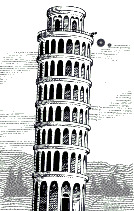
\includegraphics[width=0.5\textwidth]{pizza}
    \captionof{figure}{Caida libre.}
    \label{fig:caida}
\end{minipage}
\begin{minipage}{0.5\textwidth}
    \vspace{1.5cm}
    \centering
    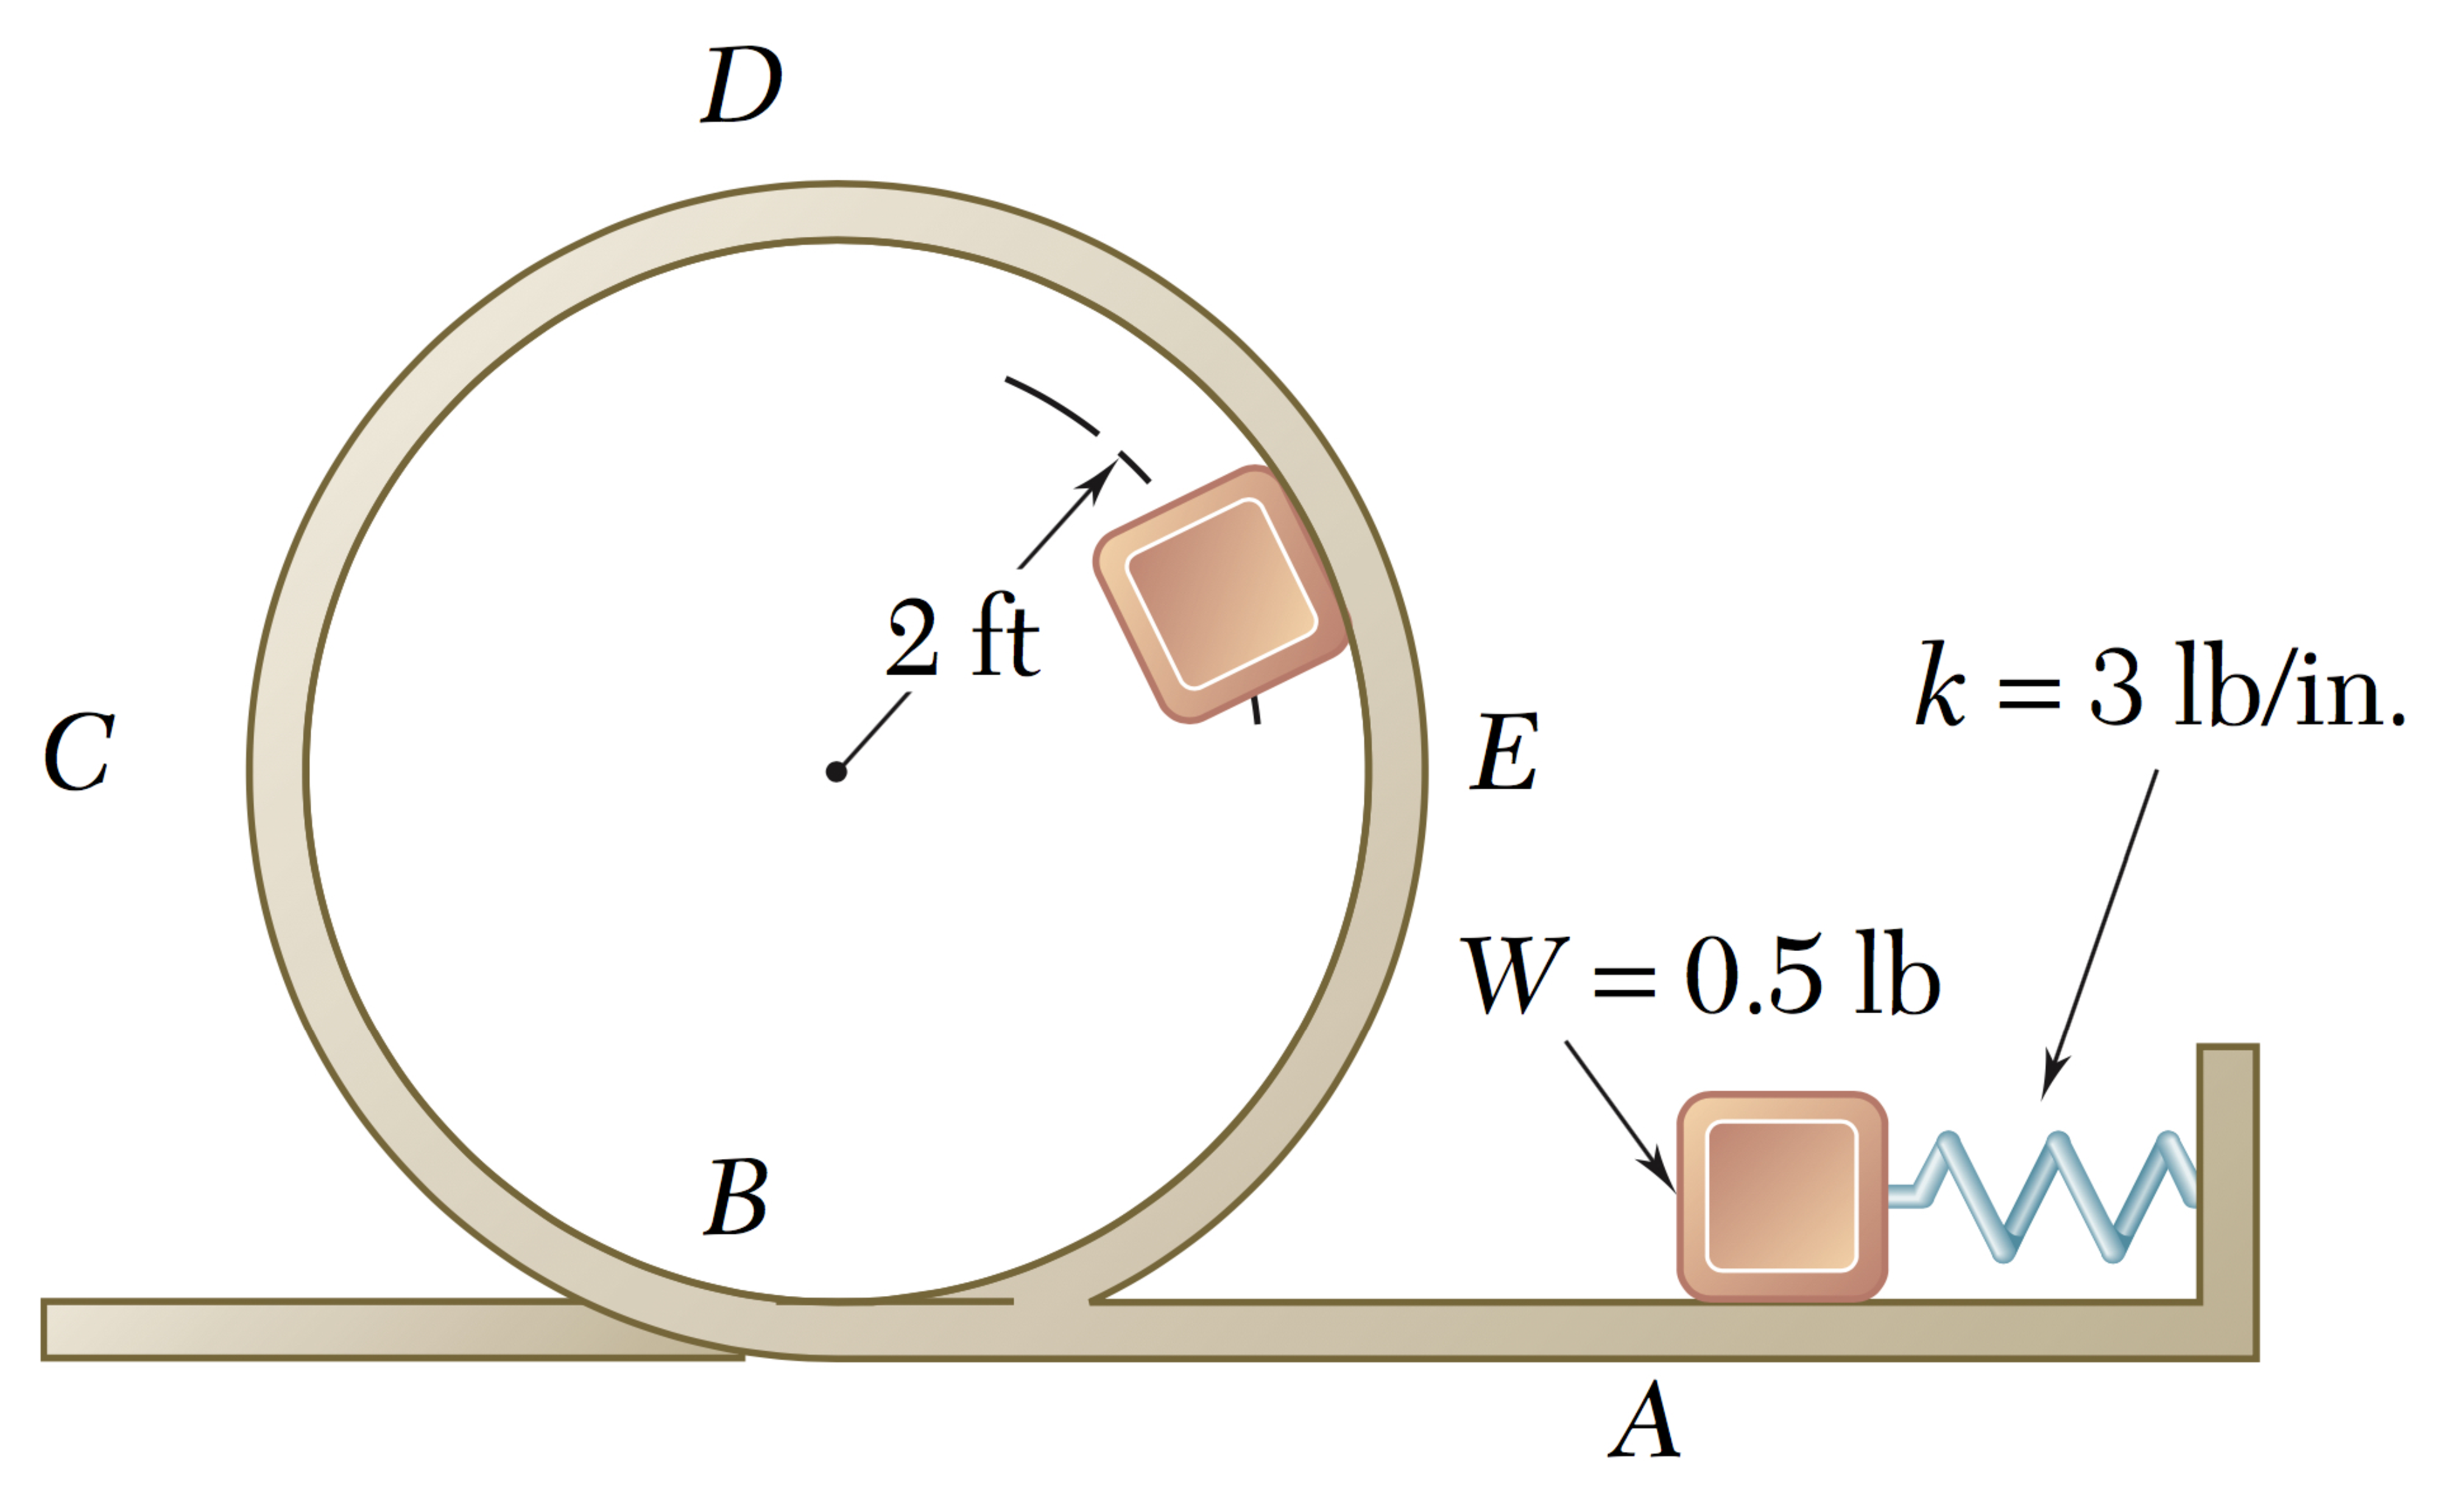
\includegraphics[width=\textwidth]{bucle}
    \captionof{figure}{Bucle.}
    \label{fig:bucle}
\end{minipage}
% section problemas (end)
\end{enumerate}

\newpage
\begin{center}
{\sc \huge Respuestas}
\end{center}

\section*{Teor\'ia} % (fold)
\label{sec:teoria2}
\begin{enumerate}

\item Un sistema de referencia inercial es quel en el cual las leyes de Newton
se cumplen. Esto implica que el mismo tenga velocidad constatne.

\item Ambos est\'an definidos como distancia recorrida por unidad de tiempo. La
velocidad es una cantidad vectorial que toma en cuenta s\'olo la posici\'on
inicial y la final. La rapidez es una cantidad escalar que toma en cuanta toda
la trayectoria.

\item La aceleración de un objeto es directamente proporcional a la fuerza neta que actúa sobre él e inversamente proporcional a su masa:
\begin{equation*}
F=ma.
\end{equation*}

\item Demostraci\'on:
\begin{align*}
F &=\frac{d}{dt}\boldsymbol{p} = \frac{d}{dt} m \boldsymbol{v} = 
\cancel{\frac{dm}{dt}} \boldsymbol{v} + m \frac{d\boldsymbol{v}}{dt} \\
  &=m \frac{d\boldsymbol{v}}{dt} = m \boldsymbol{a}
\end{align*}

\item La fuerza gravitacional ejercida por dos cuerpos con masas $m_{1}$ y
$m_{2}$ es directamente proporcional al producto de las masas e inversamente
proporcional al cuadrado de la distancia que las separa y adem\'as \'esta
act\'ua en la direcci\'on que une a ambas masas. $G$ es la constante de
proporcionalidad.

\item Componentes de un vector:
\begin{align*}
\boldsymbol{A_{x}} &= A\cos(\theta) \\
\boldsymbol{A_{y}} &= A\sin(\theta)
\end{align*}

\item Una fuerza conservativa es aquella cuyo trabajo depende \'unicamente de
las posiciones inicial y final de la part\'icula y no de la trayectoria que
\'esta ha descrito para ir desde la posici\'on inicial a la final. 

Para una fuerza discipativa, el trabajo realizado depende de la trayectoria.

\item Teorema de trabajo y energ\'ia:
\begin{align*}
T_{1} + V_{1} &= T_{2} + V_{2}  \\ \nonumber \\
\frac{1}{2}mv^{2}_{1} + mgh_{1} &= \frac{1}{2}mv^{2}_{2} + mgh_{2}
\end{align*}

\end{enumerate}

\section*{Problemas} % (fold)
\label{sec:problemas2}

% section problemas (end)

\begin{enumerate}

\item Fuerza gravitacional: 3.52$\times 10^{22}$\,N.
\hfill \textbf{8 puntos.}

\item Proyectil en tiro parab\'olico:
\hfill \textbf{9 puntos.}

(a) $x=3100$\,m,

(b) $y_{max} = 563$\,m. 

\newpage
\item Ca\'ida libre:
\hfill \textbf{8 puntos.}

$y_{i} =  44.145$\,m

$v_{f} = 29.43$\,m/s
% \begin{align*}
% \cancel{y_{f}} - y_{i} &= \cancel{v_{i}}t - \frac{1}{2}gt^{2}, \\
% y_{i} &= \frac{1}{2}gt^{2} \\
% &= 44.145\,{m}
% \end{align*}

\item Automovil acelerando
\hfill \textbf{8 puntos.}

(a) $a=10.3$\,m/s$^{2}$,

(b)U=T=865\,KJ ,

(c) 320\,KW.

\item Energ\'ia potencial $\rightarrow$ energ\'ia cin\'etica:
\hfill \textbf{8 puntos.}

$v=\sqrt{2gh} = 32.85$\,m/s.

\item Resorte:
\hfill \textbf{9 puntos.}

$x=0.33$\,ft

% section teoria (end)
\end{enumerate}
\end{document}




















